
\documentclass[preprint,12pt]{elsarticle}

\usepackage[spanish]{babel}
\usepackage{amssymb}
\usepackage{graphicx}
\usepackage{lineno}
\usepackage[utf8]{inputenc}
\usepackage{url}
\usepackage{natbib}

\begin{document}
	
	\begin{frontmatter}

		\title{\huge  Comparativa de Cuadro de Mando Integral (BSC) y Modelo de Negocio Canvas (BMC) }
		\author{Robles Flores, Anthony Richard	                (2016056192)}
		\author{Estrella Palacios, Katherine Lizbeth			(2015050948)}
		\author{Sosa Bedoya, Sharon Fiorela				(2016054460)}
		\author{Torres Beltran , Johanna Andrea			(2020067849)}
		\address{Tacna, Perú}
		


%%INICIO abstract
\begin{abstract}
The Balanced Scorecard (CMI Spanish Acronym) and the Canvas model can be linked as complementary tools for entrepreneurs. The first develops goals and operational measures in four main perspectives for the purpose of achieving the mission and strategy. The second suggest a (re-) evolution in generating business models, establishing nine sections that reflect their logic. In the article a working model is developed that, based on the need for a CMI it relates its design to the information previously collected in the Canvas model, pointing their mutual necessity
\end{abstract}
%%FIN abstract


\end{frontmatter}

%%INICIO Resumen
\section{Resumen}
El Cuadro de Mando Integral (BSC) y el modelo Canvas pueden enlazarse como herramientas complementarias para los emprendedores. La primera desarrolla objetivos y medidas operativas en cuatro perspectivas principales para alcanzar la misión y estrategia. La segunda ha supuesto una (re-)evolución en la generación de modelos de negocio, estableciendo nueve apartados que reflejan su lógica. En el artículo se desarrolla un modelo de trabajo que, partiendo de la necesidad de disponer de un BSC, relaciona su diseño con la información recogida previamente en el modelo Canvas, señalando su mutua necesidad.
%%FIN Resumen


%%INICIO Introducción
\section{Introducción}
En la literatura de dirección estratégica, el cuadro de mando integral (Balanced Scorecard, BSC de aquí en adelante) se considera como una de las herramientas más conocidas e importantes para la implementación de la estrategia. Su utilidad destaca en el momento de desarrollar objetivos operativos para la comunicación de la misión y estrategia de la empresa, así como en la medición del grado de consecución de éstas, proponiendo convertir la estrategia en un conjunto de medidas de actuación que permiten su traducción y gestión. De esta forma, un BSC ha de estar constituido por un conjunto limitado de medidas financieras y no financieras organizadas en cuatro principales perspectivas interrelacionadas entre sí (Da Silva et al., 2013), que describen la estrategia organizativa a través de relaciones causa-efecto entre los indicadores: (1) financiera, (2) cliente, (3) interna e (4) innovación y crecimiento.\\ \\

Canvas es una herramienta para la generación de modelos de negocios desarrollado por Alex Osterwalder (2004), que permite trabajar sobre la base de cómo una organización crea, proporciona y captura valor. Como indican Zott et al., (2011), aunque no hay consenso entre los académicos sobre lo que es un modelo de negocio, este concepto sí incluye una visión holística del negocio como unidad de análisis donde se enfatiza el papel de las actividades de la empresa en la generación de valor. Especialmente adecuado en la fase start-up o de búsqueda del modelo de negocio, en la que predominan la alta complejidad y la dificultad de considerar numerosas variables, el Canvas propone un lenguaje y visualización que permite describirlo fácilmente, facilitando su evolución y adaptación, de forma intuitiva, siendo fácil de usar y comprender para definir la alternativa estratégica seleccionada por la nueva empresa, donde exista una propuesta de valor que recoja, además de la importancia de los procesos internos, la relevancia de las relaciones con los diferentes stakeholders. \\ \\

En nuestro artículo vamos a desarrollar el aspecto teórico más importantes sobre ambas herramientas, así mismo realizaremos una comparativa entre el Cuadro de Mando Integral (BSC) y el Modelo de Negocio Canvas (BMC) 

%%FIN Introducción


%%INICIO Marco Teórico
\section{Marco Teórico}

%%----------------------------------------------------------------------------------------------------------------------------------------------------------
	\subsection{\textbf{Cuadro de Mando Integral (BSC)}}
	
\subsubsection{\textbf{Concepto de Cuadro de Mando Integral}}

El Cuadro de Mando Integral (CMI) o BSC por sus siglas en inglés, consiste en analizar la organización en torno a cuatro perspectivas: finanzas, cliente, procesos internos y por último, innovación y aprendizaje. Significa que las cuatro perspectivas son referidas a diferentes visiones a partir de un campo de actuación, pero la integración de las cuatro perspectivas mantiene el equilibrio.

%%En este caso el punto de partida es el término "balanced", (equilibrado o balanceado) como explican los autores Kaplan y Norton (2001:8): "El nombre refleja el equilibrio entre objetivos a corto y largo plazo, entre medidas financieras y no financieras, entre indicadores previsionales e históricos, y entre perspectivas de actuaciones externas e internas"

Podríamos definir al CMI como un sistema de medida del rendimiento que se deriva de la visión y la estrategia, y que refleja los aspectos más importantes de la organización. Por consiguiente, permitirá un monitoreo integral por el hecho de que utiliza tanto indicadores financieros como no financieros, justamente estos últimos hacen que se reconozca su utilidad al gestionar recursos intangibles, poco reconocidos y difícilmente evaluables. \cite{referenciaestrella1} 

El desarrollo del Cuadro de Mando Integral gira en torno a cinco ideas escenciales:  

	\begin{itemize}
		\item Herramienta de ayuda durante el proceso de toma de desiciones
		\item Diseño sencillo y eficaz
		\item Reune indicadores financieros y nos financieros
		\item Flexible frente a los cambios y progresos del entorno
		\item Genera motivación a todos lo niveles de responsabilidad \cite{referenciaestrella3} 
	\end{itemize}


\subsubsection{\textbf{Perspectivas del Cuadro de Mando Integral}}

Kaplan y Norton establecen las cuatro perspectivas ya mencionadas. La lógica empleada proporciona respuestas a cuatro preguntas por cada perspectiva: 

	\begin{itemize}
	\item{\textbf{1. Perspectiva financiera: }} La perspectiva financiera está orientada a maximizar los beneficios y definir los objetivos para animar a los dueños o accionistas a asegurarle fondos continuos a la organización, perspectiva que verifica el logro de los objetivos empresariales los cuales incluyen tres dimensiones fundamentales: rentabilidad, crecimiento y valor del accionista.
	\item {\textbf{2. Perspectiva del cliente: }} Se refiere al conjunto de actividades que generan valor y, por ende, aumentan la capacidad competitiva de la empresa. Tales actividades permiten ver cómo los clientes perciben el valor ofrecido, por lo que recompensarán a la organización con los resultados financieros que ésta espera obtener, pues la percepción depende de la habilidad para entregar valor y comunicar. %%También constituyen la zona medular de una estrategia bien implementada, lo que verifica hasta qué punto los clientes son fieles y se encuentran satisfechos. Intervienen en esta perspectiva cuatro importantes dimensiones: tiempo, calidad, desempeño y servicio del producto, y costo de la propiedad.
	\item {\textbf{3. Perspectiva del proceso interno: }} En esta perspectiva se identifican los procesos críticos internos en los que la organización debería ser excelente. Esto permite focalizar la entrega percibida de acuerdo con el objetivo del cliente, y analiza el proceso interno que influye directamente en la satisfacción de éste. A menudo abarca tres dimensiones: tiempo de ciclo, calidad y productividad.
	\item {\textbf{4. Perspectiva de innovación y aprendizaje: }} Constituye la base que permitirá alcanzar los objetivos de las demás perspectivas del CMI. Las organizaciones deben invertir en la capacitación, potenciar los sistemas y tecnologías de la información, y coordinar los procedimientos y rutinas del trabajo de una forma más eficiente. Participan en esto tres dimensiones: innovación de mercado, aprendizaje y mejora operacional continua, así como de activos intelectuales.  \cite{referenciaestrella2}

	\end{itemize}


	\begin{figure}[htb]
		\begin{center}
			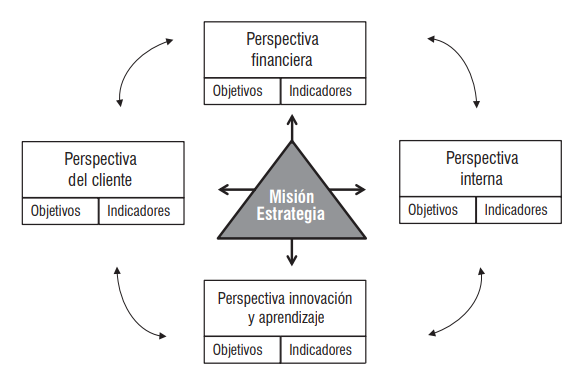
\includegraphics[height=6.5cm]{./IMAGENES/Perspectivas_BSC} 
			\caption{Perspectivas del Cuadro de Mando Integral} 
		\end{center}
	\end{figure}



\subsubsection{\textbf{Propuesta de Valor al Cliente}}

%%https://www.grandespymes.com.ar/2011/06/13/balanced-scorecard-cuadro-de-mando-integral/

Dado que el BSC ha de ser sencillo y fácilmente entendible, es clave seleccionar aquellos objetivos estratégicos de primer nivel que son prioritarios. Para ello, resulta de gran utilidad definir la propuesta de valor al cliente, es decir, lo que diferencia a nuestra organización ante los clientes. Diferentes gurús de la estrategia han distinguido formas de competir. Kaplan y Norton las resumen, siguiendo la clasificación de Trecy y Weserman, en:

	\begin{itemize}
	\item Liderazgo de productos: se centra en la excelencia de sus productos y servicios, que ofrecen la máxima calidad y funcionalidad.
	\item Relación con el cliente: se centra en la capacidad para generar vínculos con los clientes, para conocerlos y proporcionarles productos y servicios adecuados a sus necesidades.
	\item Excelencia operativa: se centra en proporcionar productos y servicios a un precio competitivo para la calidad y funcionalidad que ofrecen.
	\end{itemize}

Las organizaciones intentan ser excelentes en una de esas estrategias, manteniendo unos estándares mínimos en las otras dos. Es lógico que las perspectivas del cliente y, por ende, las  de procesos y aprendizaje y crecimiento, se centren en objetivos relacionados con la estrategia para los que no se ha conseguido el mínimo requerido.\cite{referenciarobles1} 

\subsubsection{\textbf{Indicadores y sus Metas}}

Los indicadores (también llamados medidas) son el medio que tenemos para visualizar si estamos cumpliendo o no los objetivos estratégicos.

Un objetivo estratégico, como por ejemplo el desarrollo de capacidades comerciales de nuestro personal clave, puede medirse a través de indicadores.
\\

Se pueden establecer dos tipos de indicadores:

	\begin{itemize}
	\item Indicadores de resultado: miden la consecuencia del objetivo estratégico. También se les llama indicadores de efecto.
	\item Indicadores de causa: miden el resultado de las acciones que permiten su consecución. También se llaman indicadores inductores.
	\end{itemize}

Las organizaciones intentan ser excelentes en una de esas estrategias, manteniendo unos estándares mínimos en las otras dos. Es lógico que las perspectivas del cliente y, por ende, las  de procesos y aprendizaje y crecimiento, se centren en objetivos relacionados con la estrategia para los que no se ha conseguido el mínimo requerido.\cite{referenciarobles2} 

\subsubsection{\textbf{Iniciativas Estratégicas}}

Las iniciativas estratégicas son las acciones en las que la organización se va a centrar para la consecución de los objetivos estratégicos. En nuestras empresas hacemos cosas, pero ¿están realmente enfocadas hacia el cumplimiento de la estrategia? En muchas organizaciones encontramos un exceso de iniciativas y proyectos con falta de recursos y tiempo para llevarlos a cabo.
\\

Es importante priorizar las iniciativas en función de los objetivos estratégicos. Si analizamos el impacto de las iniciativas en marcha en cada uno de los objetivos estratégicos, podemos visualizar, iniciativas que aportan poco valor al cumplimiento de estos objetivos y objetivos estratégicos sin soporte a las iniciativas\cite{referenciarobles3} 

\subsubsection{\textbf{Responsables y Recursos}}

Cada objetivo, indicador e iniciativa debe tener un responsable. Una persona a cargo que controla su cumplimiento.
\\
Otro aspecto clave para una implantación con éxito del BSC es asignar los recursos necesarios para el buen desarrollo de las iniciativas estratégicas. Es el primer paso para el cumplimiento de la estrategia. Por ello es necesario establecer los equipos a cargo de cada iniciativa, así como el papel que diferentes personas van a jugar en ellos. Y también dotar a las iniciativas de los recursos necesarios para su cumplimiento. Se recomienda que el presupuesto contenga una partida de recursos asignados a las iniciativas estratégicas. Estos recursos deben estar diferenciados del presupuesto operativo, del presupuesto de inversión y de otros presupuestos que utilizan las empresas, asi podemos evitar que otras actividades engullan esos recursos que debieran dedicarse al cumplimiento de las iniciativas críticas definidas en el BSC.\cite{referenciarobles2} 

\subsubsection{\textbf{Características del Cuadro de Mando Integral}}

El desarrollo de un sistema integral de gerencia requiere un sistema balanceado de indicadores. El sistema reconoce la causa y efecto entre acciones y resultados. Reconoce que para deleitar a un inversionista, la empresa tiene que ser rentable. Reconoce que para hacer feliz al cliente necesita reducir o eliminar costos y mejorar la calidad del producto o servicio. Para mantener la ventaja competitiva a largo plazo, es necesario aprender y aprender y a innovar. El Balanced Scorecard tiene las siguientes características:


	\begin{itemize}
	\item Articula los factores que impulsan la estrategia de la organización.
	\item Le pone brazos y manos a la visión/misión.

	\item Permite, de forma concreta, entender la razón de ser de la organización y sus metas
	\item Define en concreto las metas críticas para alcanzar el éxito.

	\item Permite su difusión a lo largo y ancho de la organización.
	\item Define el desarrollo de indicadores de desempeño para cada meta.

	\item Asegura que todos entienden los indicadores de las áreas y de la empresa en general.
	\item Comunica cómo estos están interrelacionados.

	\item Conecta cada medida a un sistema de retroalimentación formal.
	\item Integra la comunicación con la regularidad.

	\item Integra la comunicación con la regularidad.
	\end{itemize}

%%----------------------------------------------------------------------------------------------------------------------------------------------------------

	\subsection{\textbf{Modelo de Negocio Canvas (BMC) }}

El modelo de canvas es una herramienta para analizar y crear modelos de negocio de manera simplificada. Se puede ver globalmente en el lienzo, que se divide en los principales aspectos relacionados con el negocio y se centra en la propuesta de valor proporcionada. \\\\
El modelo de negocio de canvas es una herramienta que en 2010 fue dado a conocer debido al libro “Generación de modelos de negocio” (Business Model Generation) de Alex Osterwalder e Yves Pigneur. \cite{referenciasosa4}\\
La herramienta comenzó a integrarse entre los más visionarios, revolucionarios y desafiantes que querían desafiar modelos de negocios obsoletos y diseñar futuras empresas.  \cite{referenciasosa4}\\\\
El modelo de canvas se utiliza para transformar una idea en un proyecto y plasmar nuestra idea en un modelo de negocio. Este es un modelo "vivo", es decir, vamos modificando según se va desarrollando, verifiquemos a los clientes y puede surgir nuevas ideas, y es por eso que se utiliza post-it para completarlo.

	\subsubsection{\textbf{Características}}
	\begin{itemize}
	\item{\textbf{1. Práctico: }}Permite realizar diferentes cambios al analizar y testear las hipotesis más riesgoas, las que pueden poner en peligro la viabilidad del negocio.
	\item {\textbf{2. Intuitivo - Creativo: }}Su forma tan simple de ser nos permite imprimir el lienzo del modelo de negocio en tamaño XL y usar notas adhesivas y rotuladores de color.
	\item {\textbf{3. Permite Trabajar en Equipo: }}Cuelga el lienzo en la pared y hazlo visible para todos. Despeje la mesa y trabaje en grupos de una manera muy interactiva y dinámica.
	\item {\textbf{4. Visual: }}Brinda una visión global de todos los aspectos importantes que conforman el modelo de negocio. Una vez que se completa el análisis, se expone el lienzo para que todos los miembros puedan comprender claramente la visión global de la empresa de un vistazo.
	\end{itemize}

	\subsubsection{\textbf{Módulos del BMC}}
El modelo de negocio canvas se divide en nueve módulos. \\\\El lado derecho se refiere al mercado, los aspectos externos de la empresa, el entorno. Consta de las siguientes partes: segmentación del mercado, propuesta de valor, canales, relación con los clientes y fuentes de ingresos.\\\\ Los aspectos internos se reflejan a la izquierda, como asociaciones clave, actividades y recursos clave y estructuras de costos.

\begin{figure}[htb]
		\begin{center}
			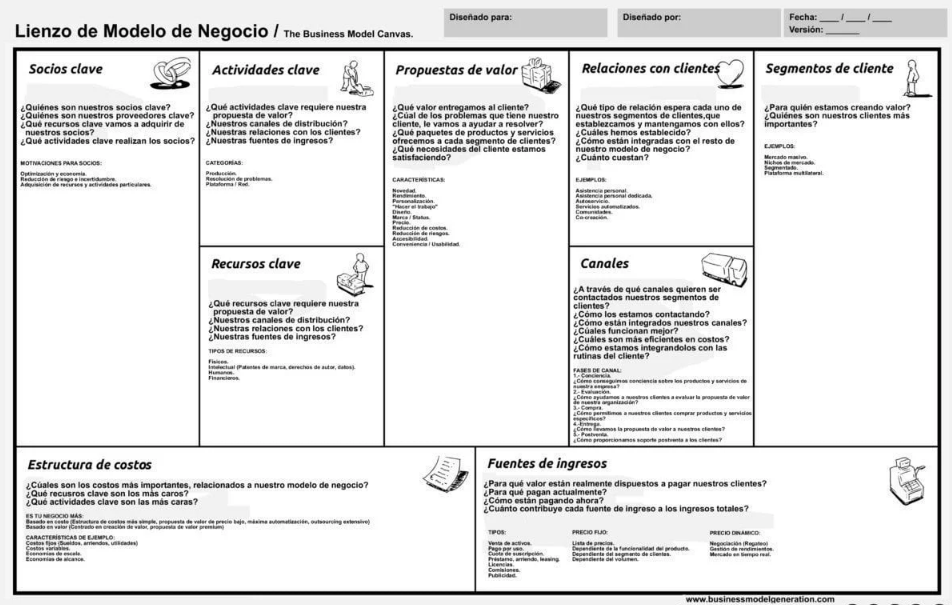
\includegraphics[height=10cm]{./IMAGENES/modeloCanvas2} 
			\caption{Módulos del Modelo de Negocio de Canvas}  \cite{referenciasosa2} 
		\end{center}
	\end{figure}

	\begin{itemize}
	\item {\textbf{Propuesta de valor: }} Es el núcleo fundamental del modelo de negocio, es decir, los productos proporcionados por la empresa para satisfacer la demanda del mercado. El valor no solo se refleja en el producto, sino también en todos los aspectos que los consumidores pueden percibir y experimentar.\cite{referenciasosa2}  \\\\Dar respuesta a estas preguntas:\\ • ¿Qué valor estamos entregando a nuestros clientes?\\ • ¿Qué problema resolvemos?\\ • ¿Cuál es la necesidad que satisfacemos? \\ • ¿Qué tipo de producto ofrecemos? 

	\item {\textbf{Segmentos de clientes: }} Su objetivo es definir los clientes típicos que las empresas intentan atraer en función de diferentes criterios, como su edad, poder adquisitivo, los bienes que compran, que compran o el lugar donde viven. \\Identificar las necesidades del mercado y las necesidades del cliente. Nuestro enfoque siempre está en los clientes, y debemos guiar nuestros productos de acuerdo con sus necesidades y deseos.\\\\Dar respuesta a estas preguntas:\\ • ¿Para quién estamos creando valor?\\ • ¿Quiénes son nuestros clientes más importantes?

	\item {\textbf{Canales: }} Una vez que se determina el cliente y la propuesta de valor que le brindamos, debemos comunicarnos con ellos. \\ Esta es una de las decisiones más importantes porque generalmente determina los beneficios. La estrategia de la entidad es llevar su propuesta de valor al mercado basándose en la experiencia del cliente que pretende lograr.\cite{referenciasosa3}  Si no nos conocen, no nos comprarán. Aquí definiremos el canal de distribución del producto o servicio.\\\\Dar respuesta a estas preguntas:\\ • ¿Con qué canales podemos llegar a nuestros clientes? \\ • ¿Qué canales funcionan mejor? \\ • ¿Cuáles de estos canales son los más rentables?

	\item {\textbf{Relación con clientes: }} Esta parte se ve cada vez más afectada por la reputación de la empresa o su percepción entre la sociedad. Involucra la forma en que trata de retener y fidelizar clientes, y la relación entre el cliente y la compañía. Es el tipo de comunicación que se desea establecer con cada segmento de clientes para mantenerlo y lograr el posicionamiento esperado gracias a la propuesta de valor.  \\\\Dar respuesta a estas preguntas:\\ • ¿Cuál es la relación que tenemos con cada uno de nuestros segmentos de clientes? \\ • ¿Qué tipo de relación esperan? \\ • ¿Qué coste tiene?

	\item {\textbf{Fuentes de ingresos: }} El elemento básico para garantizar la viabilidad económica del negocio, ya que implica cómo la empresa pretende cobrar por productos y servicios a través del pago y otros métodos. \\\\Dar respuesta a estas preguntas:\\ • ¿Cuál es nuestra principal línea de ingresos?\\ • ¿Cómo pagarán nuestros clientes? \\ • ¿Por qué están dispuestos a pagar nuestros clientes? 

	\item {\textbf{Recursos clave: }} Conocer con qué recursos contamos y con los que debemos contar para llevar a cabo la actividad de nuestro negocio, es clave a la hora de establecer el plan de negocios. Este módulo integra todo el contenido que la empresa utiliza para llevar a cabo sus actividades, como la colocación de productos en el mercado, la generación de ingresos o las relaciones que mantiene con las partes interesadas y los clientes.\cite{referenciasosa3} \\\\Dar respuesta a estas preguntas:\\ • ¿Qué recursos esenciales requiere nuestra propuesta de valor?
	\item {\textbf{Actividades clave: }}Para llevar a cabo la propuesta de valor que queremos ofrecer a nuestros clientes, son necesarias ciertas actividades para preparar el producto antes de que llegue al mercado. \\Son todas las acciones, tareas y procesos necesarios para proporcionar valor a las cotizaciones existentes en el mercado. Entre ellos, destacan la asistencia posventa, marketing, transporte o distribución.\cite{referenciasosa3}  \\\\Dar respuesta a estas preguntas:\\ • ¿Qué actividad básica requiere nuestra propuesta de valor? \\ • ¿Cuáles son nuestros canales? \\ • ¿Cuáles son nuestras fuentes de ingresos?

	\item {\textbf{Socios clave: }} Para llevar a cabo un negocio, es imprescindible tener aliados.\cite{referenciasosa1}  Estos aliados pueden ser: Socios, colaboradores, proveedores. Analiza proveedores y agentes adecuados y necesarios para poder ejecutar con éxito todos los procesos. A través de ellos, se pueden establecer diversos acuerdos y alianzas para garantizar el mantenimiento a largo plazo de las actividades de la empresa. \\\\Dar respuesta a estas preguntas:\\ • ¿Quiénes son nuestros socios clave en el mercado? \\ • ¿Quiénes son nuestros proveedores?
	\item {\textbf{Estructura de costes: }}El objetivo principal de cualquier entidad es garantizar su sostenibilidad. Por lo tanto, es importante evaluar todos los costos fijos del negocio y elegir el costo más apropiado en términos de eficiencia y rentabilidad. \\ Tener bien clara esta estructura nos ayudará a no desviarnos de los presupuestos y que el negocio fracase por problemas de financiación.\cite{referenciasosa1}  \\\\Dar respuesta a estas preguntas:\\ •  ¿Cuáles son los costes más importantes dentro de nuestro modelo de negocio?\\ •  ¿Qué recursos clave son los más costosos? \\ • ¿Qué actividades clave son las más costosas?
	\end{itemize}

	\subsubsection{\textbf{Beneficios del Uso de BMC}}
Este modelo de negocio de canvas fomenta nuevas formas de crear, entregar y captar valor para el cliente mediante el aprendizaje validado. Sus beneficios encontrados son:
\begin{itemize}
	\item{\textbf{1. Mejora la comprensión: }}Utiliza herramientas visuales. Este método fomenta el pensamiento creativo de los trabajadores que crean el lienzo.
	\item {\textbf{2.Amplios puntos de enfoque: }}El modelo mantiene la misma visión del modelo de negocio desde diferentes perspectivas: negocio, mercado, canales de distribución, etc.
	\item {\textbf{3. Análisis estratégico: }}En solo una hoja se pueden visionar todos los elementos del lienzo. Una forma sencilla para sacar el mayor partido a esta herramienta.
	\end{itemize}




%%FIN Marco Teórico
%%----------------------------------------------------------------------------------------------------------------------------------------------------------


%COMPRACION

\section{Comparación entre Cuadro de Mando Integral (BSC) y Modelo de Negocio Canvas (BMC)}
A continuación se muestra la comparación entre Cuadro de Mando Integral (BSC) y Modelo de Negocio Canvas (BMC)
	
	\begin{itemize}

	\item{\textbf{1.}} El cuadro de mando integral se utilizan para monitorear el desempeño de la organización a lo largo del tiempo. Si se observa una caída estadística en el puntaje,
	 la organización debe iniciar un cambio para detener la disminución del rendimiento. Mientras que el  modelo de negocio Canvas se utiliza como una herramienta de diagnóstico como
 una lente en el estado actual del negocio, especialmente las cantidades relativas de energía, tiempo y recursos que actualmente se invierten en diversas áreas. Si alguna de las áreas del modelo no funciona bien, la organización debe iniciar un cambio para mejorarla.
	\item{\textbf{2.}}Balanced Scorecard evolucionó a una encarnación de "mapas estratégicos", que era un enfoque más visual similar al Business Model Canvas. Sin embargo, el Business Model Canvas tiene un mayor potencial alcista aquí porque es mucho más intuitivo y requiere menos explicación.
	\item{\textbf{3.}}El mando de cuadro integral se encuentran cuatro perspectivas que son referidas a diferentes visiones a partir de un campo de actuación, pero la integración de las cuatro perspectivas mantiene el equilibrio. Mientras que el modelo de negocio canvas que se divide en los principales aspectos relacionados con el negocio y se centra en la propuesta de valor proporcionada.
	\item{\textbf{4.}} BSC y el modelo de negocio canvas buscan expresar o reflejar el modelo de negocio de una organización.
	\item{\textbf{5.}}BSC que habla de la perspectiva de Procesos y la fundamenta en la CADENA DE VALOR (Producción), el CANVAS al ser más reciente, ha incorporado el concepto de Configuraciones de Valor con el nombre Actividades Claves y las clasifica en tres; Actividades de Producción es decir las que se manejan con CADENA DE VALOR, Actividades de resolución de problemas (Servicios) que se manejan con CICLO DE VALOR y las actividades de plataforma o red que se manejan con RED DE VALOR.
	\item{\textbf{6.}} BSC le da gran impirtancia a la Tecnología Informática mientras que en el modelo de negocio CANVAS habría que verla en los recursos físicos e intelectuales.
	\item{\textbf{7.}}El corazón del Canvas es la Propuesta de Valor, que correspondería a la perspectiva del Cliente en el Balanced Scorecard y es donde el Canvas, desarrolla más elementos; deja explícito que para llegar a los clientes debo definir cuál tipo de relación voy a tener con ellos y que canales voy a utilizar.
	\end{itemize}

%%----------------------------------------------------------------------------------------------------------------------------------------------------------

%CONCLUSIONES
\section{Conclusiones}

%%****
	\begin{itemize}
		\item El cuadro de mando integral junto con el modelo de negocio canvas trabajan en equipo para lograr su objetivo, ya que se divide en varios aspectos y es necesario cada participante del equipo de su punto de vista de tal froma que se llegan a la  idea en especifica y de esa manera empezar a trabajar sobre ese objetivo planteado.
		\item El cuadro de mando integral 
		\item XXXXXXXXXXXXXXXXXXXX
	\end{itemize}

%%----------------------------------------------------------------------------------------------------------------------------------------------------------

%RECOMENDACIONES
\section{Recomendaciones}	

	\begin{itemize}
		\item Conocer ampliamente la metodología que se va trabajar.
		\item En las dos metodologías que se nombraron anteriormente es de vital importancia trabajar en conjunto con los departamentos de organización.
		\item Es necesario se claro, concreto y tener criterio a la hora de definir lo bueno y lo malo de la organización.
	\end{itemize}


%%----------------------------------------------------------------------------------------------------------------------------------------------------------

	
	\newpage
	\bibliographystyle{apalike}
	\bibliography{BIBLIOGRAFIA}	


\end{document}

